\documentclass{article}
\usepackage[utf8]{inputenc}
\usepackage[letterpaper, margin=1in]{geometry}
\usepackage{amsmath}
\usepackage{tikz}
\usepackage{pgfplots}
\usepackage{amssymb }

\title{CS5780 HW4}
\author{Renhao Lu, NetID: rl839}
	
\begin{document}
	\maketitle
	
	\section{Problem: Linear Regression}
	\subsection{Compute the closed form solution for $\textbf{w}$}
	Using the formula in class:
	\[
	\textbf{w} = 
		(\textbf{X} \textbf{X}^T) ^{-1}
		\textbf{X}
			\textbf{y}^T
	\]
	where $\textbf{X}=\begin{pmatrix} 1 & 1 & 1 & 1 & 1 \\ -1 & 0 & 1 & 2 & 3\end{pmatrix}$ and  $\textbf{y}=\begin{pmatrix} 4 & 3 & -4& 3 & 7 \end{pmatrix}$\\
	Hence,
	\[\begin{split}
		\textbf{w}&=(\textbf{X}\textbf{X}^T)^{-1}\textbf{X}\textbf{y}^T\\
		&=\begin{pmatrix} 5 & 5 \\ 5 & 15\end{pmatrix}^{-1}\textbf{X}\textbf{y}^T\\
		&=\begin{pmatrix} 0.3 & -0.1 \\ -0.1 & 0.1\end{pmatrix}\textbf{X}\textbf{y}^T\\
		&=\begin{pmatrix} 0.4 & 0.3 & 0.2 & 0.1 & 0 \\ -0.2 & -0.1 & 0 & 0.1 & 0.2\end{pmatrix}\textbf{y}^T\\
		&=\begin{pmatrix} 2 \\ 0.6\end{pmatrix}
	\end{split}\]
	
	\subsection{Calculate the training loss}
	\[
		\begin{split}
			l(\textbf{w})&=\sum (y_i-\textbf{w}^T\phi(x_i)^2)\\
			&={||\textbf{y}-\textbf{w}^textbf{X}||}_2^2\\
			&={||\begin{pmatrix} 2.6 & 1 & -6.6 & -0.2 & 3.2 \end{pmatrix}||}_2^2\\
			&=61.6
		\end{split}
	\]
	
	\section{Problem: Linearity of Gaussian Naive Bayes}
	\subsection{Show that the decision rule}
	According to the law of total probability:
	\[
		\begin{split}
			p(\textbf{x}) &= p(y=1)p(\textbf{x}|y=1)+p(y=0)p(\textbf{x}|y=0)\\
			&=p(y=1)\prod_{\alpha=1}^d {p([\textbf{x}]_{\alpha}|y=1)} +p(y=0)\prod_{\alpha=1}^d {p([\textbf{x}]_{\alpha}|y=0)}
		\end{split}
	\]
	Hence,
	\[
		\begin{split}
			p(y=1|\textbf{x}) &=\frac{
				p(y=1) 
				\prod_{\alpha=1}^d {
					p([\textbf{x}]_{\alpha}|y=1)
				} 
			}{
				p(\textbf{x})
			} \\
			&=\frac{
				p(y=1)\prod_{\alpha=1}^d {
					p([\textbf{x}]_{\alpha}|y=1)
				}
			}{
				p(y=1)\prod_{\alpha=1}^d {
					p([\textbf{x}]_{\alpha}|y=1)
				}
				+p(y=0)\prod_{\alpha=1}^d {
					p([\textbf{x}]_{\alpha}|y=0)
				}
			}
		\end{split}
	\]
	
	\subsection{Show how to rewrite}
	From the formula we got from 1:
	\[
		\begin{split}
			p(y=1|\textbf{x}) 
			&=\frac{
				p(y=1)\prod_{\alpha=1}^d {
					p([\textbf{x}]_{\alpha}|y=1)
				}
			}{
				p(y=1)\prod_{\alpha=1}^d {
					p([\textbf{x}]_{\alpha}|y=1)
				}
				+p(y=0)\prod_{\alpha=1}^d {
					p([\textbf{x}]_{\alpha}|y=0)
				}
			}\\
			&=\frac{1}{
				1 + \frac{
					p(y=0)\prod_{\alpha=1}^d {
						p([\textbf{x}]_{\alpha}|y=0)
					}
				}{
					p(y=1)\prod_{\alpha=1}^d {
						p([\textbf{x}]_{\alpha}|y=1)
					}
				}
			}\\
			&=\frac{1}{
				1 + exp(
					-log(
						\frac{
							p(y=1)\prod_{\alpha=1}^d {
								p([\textbf{x}]_{\alpha}|y=1)
							}
						}{
							p(y=0)\prod_{\alpha=1}^d {
								p([\textbf{x}]_{\alpha}|y=0)
							}
						}
					)
				)
			}\\
		\end{split}
	\]
	\subsection{Show that Naive Bayes is a linear model}
	Because
	\[
		p([\textbf{x}]_{\alpha}|y=1)=
		\frac{1}{\sqrt{2\pi[\sigma_{\alpha}]}}
		\exp\left({
			\frac{
			-([\textbf{x}]_{\alpha}-[\mu_1]_{\alpha})^2
			}{
				2[\sigma]_{\alpha}
			}
		}\right)
	\]
	\[
		p([\textbf{x}]_{\alpha}|y=0)=
		\frac{1}{\sqrt{2\pi[\sigma_{\alpha}]}}
		\exp\left({
			\frac{
			-([\textbf{x}]_{\alpha}-[\mu_0]_{\alpha})^2
			}{
				2[\sigma]_{\alpha}
			}
		}\right)
	\]
	Hence,
	\[
		\begin{split}
			p(y=1|\textbf{x})&=\frac{1}{1+\frac{p(y=0)}{p(y=1)}\exp{\left(\sum_{\alpha=1}^d{-\log{\frac{p([\textbf{x}]_\alpha|y=1)}{p([\textbf{x}]_\alpha|y=0)}}}\right)}}\\
			&=\frac{1}{1+\frac{p(y=0)}{p(y=1)}\exp{\left(\sum_{\alpha=1}^d{\frac{([\textbf{x}]_{\alpha}-[\mu_0]_{\alpha})^2-([\textbf{x}]_{\alpha}-[\mu_1]_{\alpha})^2}{2[\sigma]_{\alpha}}}\right)}}\\
			&=\frac{1}{1+\frac{p(y=0)}{p(y=1)}\exp{\left(\sum_{\alpha=1}^d{\frac{2([\mu_1]_{\alpha}- [\mu_0]_{\alpha})[\textbf{x}]_{\alpha}+([\mu_0]_{\alpha}^2-[\mu_1]_{\alpha}^2)}{2[\sigma]_{\alpha}}}\right)}}
		\end{split}
	\]
	We assume:
	\[\textbf{w}=[w_1, w_2,...,w_b], w_\alpha=\frac{[\mu_1]_{\alpha}- [\mu_0]_{\alpha}}{[\sigma]_{\alpha}}\]
	\[b=\sum{b_\alpha}+b_0, b_0=\log{\frac{p(y=0)}{p(y=1)}}, b_\alpha=\frac{[\mu_0]_{\alpha}^2-[\mu_1]_{\alpha}^2}{2[\sigma]_{\alpha}}\]
	Hence,
	\[\begin{split}
		p(y=1|\textbf{x})&=\frac{1}{1+\exp{\left(b_0+\sum_{\alpha=1}^d {(w_\alpha[\textbf{x}]_\alpha+b_\alpha)}\right)}}\\
		&=\frac{1}{1+\exp{\left(\textbf{w}^T\textbf{x}+b\right)}}
	\end{split}\]
	From the formula above, whether $p(y=1|\textbf{x}) > p(y=0|\textbf{x})$ is decided by whether $\textbf{w}^T\textbf{x}+b>0$, hence this Naive Bayes is a linear model.
	
	\section{Problem: Gradient for Logistic Regression}
	\subsection{Show the sigmoid function property}
	\[\begin{split}
		\sigma(s)+\sigma(-s)&=\frac{1}{1+e^{-s}}+\frac{1}{1+e^{s}}\\
		&=\frac{e^s}{1+e^{s}}+\frac{1}{1+e^{s}}=1
	\end{split}\]
	Hence, $\sigma(-s)=1-\sigma(s)$
	
	\subsection{Compute the gradient of the log likelihood function}
	\subsubsection{first derivative}
	\[\sigma'(s)=-\frac{1}{(1+e^{-s})^2}(-e^{-s})=\frac{1}{1+e^{-s}}\frac{1}{1+e^s}=\sigma(s)\sigma(-s)=\sigma(s)(1-\sigma(s))\]

	\subsubsection{Show the gradient of the log likelihood function}
	\[
	\begin{split}
		\nabla_w\log(\textbf{y}|X, \textbf{w})&=\nabla_w\sum_{i=1}^n{\log\sigma(y_i(\textbf{w}^T\textbf{x}_i))}\\
		&=\sum_{i=1}^n {[\frac{\partial}{\partial w_1}\log\sigma(y_i(\textbf{w}^T\textbf{x}_i))...\frac{\partial}{\partial w_d}\log\sigma(y_i(\textbf{w}^T\textbf{x}_i))]}
	\end{split}
	\]
	Considering that,
	\[
		\frac{\partial}{\partial w_\alpha}\log\sigma(y_i(\textbf{w}^T\textbf{x}_i)) = \frac{1}{\sigma(y_i(\textbf{w}^T\textbf{x}_i))}\sigma'(y_i(\textbf{w}^T\textbf{x}_i))y_i\frac{\partial}{\partial w_\alpha}\textbf{w}^T\textbf{x}_i=(1-\sigma(y_i(\textbf{w}^T\textbf{x}_i)))y_i\textbf{x}_{i\alpha}
	\]
	Hence,
	\[\nabla_w\log(\textbf{y}|X, \textbf{w})=\sum_{i=1}^n {(1-\sigma(y_i(\textbf{w}^T\textbf{x}_i)))y_i\textbf{x}_{i}}\]
	
	\subsubsection{the weights are in the span of the feature vectors}
	Assume in $k^{th}$ iteration, the step size is $t_k$\\
	Proof by induction:\par
	Base case: in the $0^{th}$ iteration, $\textbf{w}_0=\textbf{0}=\sum_{i=1}^n0\times\textbf{x}_i$\par
	Induction assumption: assume in $k-1^{th}$ iteration, $\textbf{w}_{k-1}=\sum_{i=1}^nc_{(k-1)i}\textbf{x}_i$, then $\textbf{w}_{k}=\textbf{w}_{k-1}+t_k\nabla_w\log(\textbf{y}|X, \textbf{w})=\textbf{w}_{k-1}+t_k\sum_{i=1}^n {(1-\sigma(y_i(\textbf{w}^T\textbf{x}_i)))y_i\textbf{x}_{i}}$. We note $c_{ki}=c_{(k-1)i}+t_k(1-\sigma(y_i(\textbf{w}^T\textbf{x}_i)))y_i$, then $\textbf{w}_{k}=\sum_{i=1}^nc_{ki}\textbf{x}_i$\par
	Hence, at every iteration of gradient descent, the weights are in the span of the feature vectors.\par
	
	\section{Problem: Optimization with Gradient Descent}
	\subsection{Perform 3 steps of gradient descent}
	$f'(w)=6(w-3)$, hence $w_k=w_{k-1}-\frac 1 \alpha f'(w_{k-1})=w_{k-1}-\frac 1 2 (w_{k-1}-3)$.
	\[\begin{split}
		&w_0=5, f(w_0)=3\times2^2=12\\
		&w_1=5-\frac 1 2\times 2=4, f(w_1)=3\times1^2=3\\
		&w_2=4-\frac 1 2\times 1=3.5, f(w_2)=3\times0.5^2=0.75\\
		&w_3=3.5-\frac 1 2\times 0.5=3.25, f(w_3)=3\times0.25^2=0.1875
	\end{split}\]
	\begin{center}
		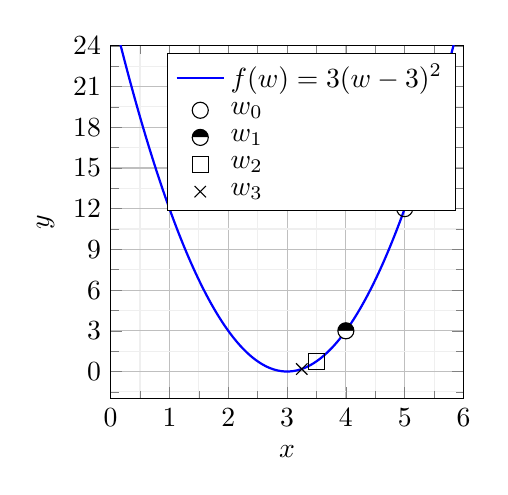
\begin{tikzpicture}
			\begin{axis}[
				xmin = 0, xmax = 6,
				ymin = -2, ymax = 24,
				xtick distance = 1,
				ytick distance = 3,
				grid = both,
				minor tick num = 1,
				major grid style = {lightgray},
				minor grid style = {lightgray!25},
				width =  .5\textwidth,
				height = .5\textwidth,
				xlabel = {$x$},
				ylabel = {$y$},
				legend cell align = {left},
			]
				\addplot[
					domain = 0:6,
					samples = 200,
					smooth,
					thick,
					blue,
				] {3*(x-3)^2};
				\addplot [only marks, mark=o,mark size=2.9pt] table {
					5 12
				};
				\addplot [only marks, mark=halfcircle*,mark size=2.9pt] table {
					4 3
				};
				\addplot [only marks, mark=square,mark size=2.9pt] table {
					3.5 0.75
				};
				\addplot [only marks, mark=x,mark size=2.9pt] table {
					3.25 0.1825
				};
				\legend{$f(w) = 3(w-3)^2$,$w_0$,$w_1$,$w_2$,$w_3$}
			\end{axis}
		\end{tikzpicture}
		\end{center}
	
	\subsection{Gradient descent can sometimes fail to converge}
	$f'(w)=20(w-11)^3$, hence $w_k=w_{k-1}-\frac 1 \alpha f'(w_{k-1})=w_{k-1}-\frac 1 2 (w_{k-1}-11)^3$.
	\[\begin{split}
		&w_0=13, f(w_0)=5\times2^4=80\\
		&w_1=13-\frac 1 2\times 2^3=9, f(w_1)=5\times2^4=80\\
		&w_2=9-\frac 1 2\times (-2)^3=13, f(w_2)=5\times2^4=80\\
		&w_3=13-\frac 1 2\times 2^3=9, f(w_3)=5\times2^4=80\\
		&...
	\end{split}\]
	The gradient descent is bouncing between $9$ and $13$ and will never converge.
	\begin{center}
		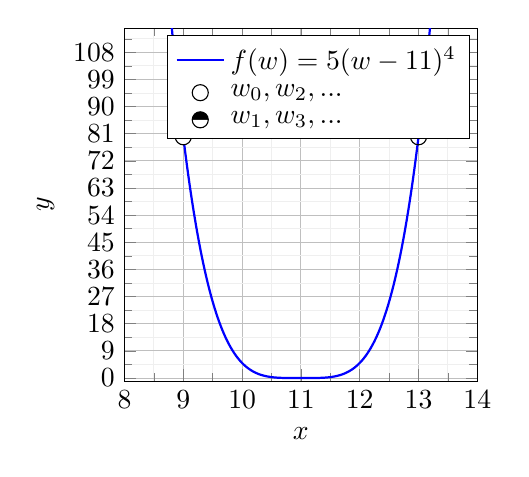
\begin{tikzpicture}
			\begin{axis}[
				xmin = 8, xmax = 14,
				ymin = -1, ymax = 116,
				xtick distance = 1,
				ytick distance = 9,
				grid = both,
				minor tick num = 1,
				major grid style = {lightgray},
				minor grid style = {lightgray!25},
				width =  .5\textwidth,
				height = .5\textwidth,
				xlabel = {$x$},
				ylabel = {$y$},
				legend cell align = {left}
			]
				\addplot[
					domain = 8:14,
					samples = 200,
					smooth,
					thick,
					blue,
				] {5*(x-11)^4};
				\addplot [only marks, mark=o,mark size=2.9pt] table {
					13 80
				};
				\addplot [only marks, mark=halfcircle*,mark size=2.9pt] table {
					9 80
				};
				\legend{$f(w) = 5(w - 11)^4$, ${w_0,w_2,...}$,${w_1,w_3,...}$}
			\end{axis}
		\end{tikzpicture}
		\end{center}
	
	\section{Problem: Derivation for Hard-margin Linear SVMs}
	\subsection{Prove the optimal solution of formulation A is a feasible solution for formulation B}
	Note the optimal solution of frmulation A is $\textbf{w}_A$. Then $\forall_iy_i(\textbf{w}_A^T\textbf{x}_i+b)\geq 0$ and $min_i|\textbf{w}_A^T\textbf{x}_i+b|=1$. Because $y_i=1or-1$, $min_iy_i(\textbf{w}_A^T\textbf{x}_i+b)=1$. Hence, $\forall_iy_i(\textbf{w}_A^T\textbf{x}_i+b)\geq 1$. $\textbf{w}_A$ is a feasible solution for B.$\blacksquare$
	\subsection{Prove the optimal solution of formulation B is a feasible solution for formulation A}
	Note the optimal solution of frmulation B is $\textbf{w}_B$, then $\forall_i,y_i(\textbf{w}_B^T\textbf{x}_i+b)\geq1$. Then obviously $\forall_iy_i(\textbf{w}_B^T\textbf{x}_i+b)\geq0$. Now we need to consider $min_i|\textbf{w}_B^T\textbf{x}_i+b|$\par
	We can prove $min_i|\textbf{w}_B^T\textbf{x}_i+b|=1$ by contradiction. We assume $min_i|\textbf{w}_B^T\textbf{x}_i+b|=p>1$, then we use a new weight vector $\textbf{w}_B'=\frac{\textbf{w}_B}{p}$. Because $p>1$, $\textbf{w}_B'^T\textbf{w}_B'=\frac{\textbf{w}_B^T\textbf{w}_B}{p^2}<\textbf{w}_B^T\textbf{w}_B$ And $\forall_i,y_i(\textbf{w}_B'^T\textbf{x}_i+b)\geq\frac p p=1$. Then $\textbf{w}_B$ cannot be optimal because $\textbf{w}_B'$ is better. $\blacksquare$
	
	\subsection{Prove that for the optimal solution in formulation A is the optimal solution for formulation B and vice versa}
	We note $\textbf{w}_A$ as the optimal solution in A, and $\textbf{w}_B$ as the optimal solution in B. From the previous questions, we know that $\textbf{w}_A$ is a feasible solution for B, so $\textbf{w}_A\leq\textbf{w}_B$. Similiarly, $\textbf{w}_B$ is also a feasible solution for A, so $\textbf{w}_B\leq\textbf{w}_A$. Hence $\textbf{w}_B=\textbf{w}_A\blacksquare$
\end{document}